\documentclass[a4paper,12pt]{ltjsreport}

\usepackage{comment}
\usepackage{float}
\usepackage{color}
\usepackage{multicol}
\usepackage{pict2e}
\usepackage{wrapfig}
\usepackage{bm}
\usepackage{url}
\usepackage{underscore}
\usepackage{colortbl}
\usepackage{tabularx}
\usepackage{fancyhdr}
\usepackage{cite}
\usepackage{amsmath,amssymb,amsfonts}
\usepackage{algorithmic}
\usepackage{textcomp}
\usepackage[utf8]{inputenc}
\usepackage{titlesec}
\usepackage[top=10truemm,bottom=30truemm,left=25truemm,right=25truemm]{geometry}%余白設定
\usepackage{hyperref,graphicx}
\usepackage{chemmacros}
\usepackage{subcaption}
\usepackage{chemfig}
\usepackage[version=3]{mhchem}  
\usepackage{braket}
\usepackage{mathtools}
\usepackage{url}
\usepackage{wrapfig}

% 新しい関数を定義
\newcommand{\vectxy}[2]{\begin{pmatrix}#1\\#2\end{pmatrix}}
\newcommand{\vectxyz}[3]{\begin{pmatrix}#1\\#2\\#3\end{pmatrix}}
\newcommand{\vectxyzw}[4]{\begin{pmatrix}#1\\#2\\#3\\#4\end{pmatrix}}
\newcommand{\vectxyzwu}[5]{\begin{pmatrix}#1\\#2\\#3\\#4\\#5\end{pmatrix}}
\newcommand{\tvectxy}[2]{\begin{pmatrix}#1 & #2\end{pmatrix}}
\newcommand{\red}[1]{{\color{red}#1}}
\newcommand{\ketvec}[1]{\ensuremath{\Ket{#1}}}
\newcommand{\con}[1]{\ensuremath{#1}}
\newcommand{\tensor}[2]{\ensuremath{{#1}\otimes{#2}}}
\newcommand{\tensorket}[2]{\ensuremath{\Ket{#1}\otimes\Ket{#2}}}
\newcommand{\tensorkets}[3]{\ensuremath{\Ket{#1}\otimes\Ket{#2}\otimes\Ket{#3}}}
\newcommand{\absquare}[1]{\ensuremath{\left|#1\right|^{2}}}
\newcommand{\braketvec}[2]{\ensuremath{\Braket{#1|#2}}}
\newcommand{\paren}[1]{\ensuremath{\left(#1\right)}}
\newcommand{\bell}[1]{\ensuremath{\Ket{{#1}^{\pm}}}}
\newcommand{\maru}[1]{\textcircled{\scriptsize #1}}
\newcommand{\redbf}[1]{\textbf{\color{red}#1}}
\newcommand{\wave}{\ensuremath{\sim}}
\newcommand{\vecb}[1]{\ensuremath{\bm{#1}}}
\newcommand{\vecbsuf}[2]{\ensuremath{\bm{#1}_{#2}}}

 %箇条書き(数字)をカッコを変更
\renewcommand{\labelenumi}{(\arabic{enumi})}

%箇条書き(記号)の記号を変更
\renewcommand{\labelitemii}{$\circ$}
\renewcommand{\labelitemiii}{$\triangleright$}

%目次にページジャンプのリンクを挿入
\hypersetup{
  setpagesize=false,
  bookmarksnumbered=true,
  bookmarksopen=true,
  colorlinks=true,
  linkcolor=black,
  citecolor=black,
}

\begin{document}
\section*{Machine Learning}
\subsection*{Introduction}
\begin{itemize}
  \item ML is subset of arrificail intelligence(AI). Deep Learning is subset of ML.
        \begin{figure}[H]
          \centering
          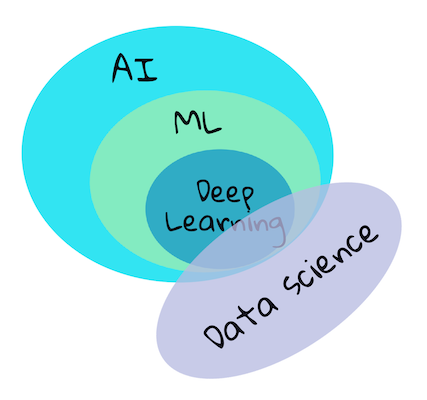
\includegraphics[keepaspectratio,scale=1]{ai-ml-ds.png}
        \end{figure}
  \item Process of creating Machine Learning
        \begin{enumerate}
          \item Decide on the question
          \item Collect and prepare data
          \item Choose a training method
          \item Train the model
          \item Evaluate the model
          \item Predict
        \end{enumerate}
  \item Building a model
        \begin{itemize}
          \item Decide on a training method by from several different training methods
          \item Train a model (model fitting)
          \item Evaluate the model by using test data
        \end{itemize}
  \item Underfitting is the problem because of unsufficient training
  \item Overfitting is the problem because of being tarined too well
        \begin{figure}
          \centering
          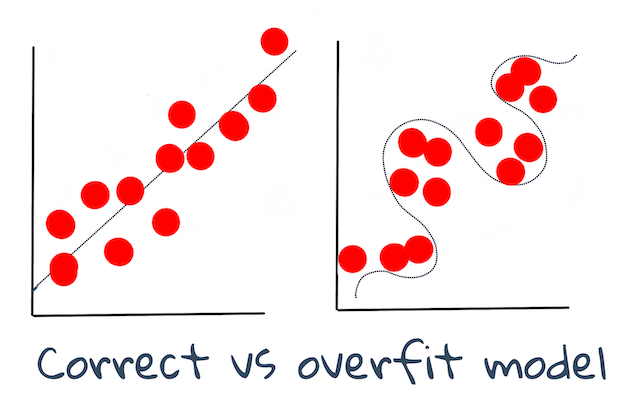
\includegraphics[keepaspectratio,scale=1]{overfitting.png}
        \end{figure}
\end{itemize}
\subsection*{Regression}
\begin{itemize}
  \item Regression model can help determine the relationship between variables
  \item The major three types of regression are linear, polynomial and logistic regression
  \item Preparation of data
        \begin{itemize}
          \item What type of ML algorithms we need depends on our question for data
          \item The quality of answer for question depends on the nature data
          \item 
        \end{itemize}
\end{itemize}
\end{document}

